\documentclass[ams]{U-AizuGT}


\usepackage{pifont}
\usepackage[dvipdfmx]{graphicx}
\usepackage{cite}
\usepackage{algorithm}
\usepackage{algpseudocode}
\usepackage{subcaption}

\bibliographystyle{ieice}


\author{Shingo Ito}
\studentid{1200045}
\supervisor{Pierre-Alain Fayolle}

\title{A simple approach to mesh deformation}


\begin{document}

\maketitle

\begin{abstract}
% (5)
In this paper, such as self-intersection for example. In order to overcome this difficulty, We suggested a more efficient deformation and reconstruction algorithm. The algorithm deform the point cloud data instead of deforming the mesh. 
\end{abstract}

\section*{Keywords:}
Mesh processing; Mesh deformation; Surface reconstruction


\section{Introduction}
% (3) Introduce the domain (mesh processing and deformation)
% justify why this problem is worth being investigated
% present an overview of the method
Mesh processing and mesh deformation is an important research topic in the geometric modeling community, with important practical applications. It allows users with relatively little technical knowledge to model complex freeform shapes through simple and intuitive interfaces. Shape deformation is a challenging topic because it can require complex mathematical formulations to be implemented as efficient (in terms of speed) computer programs.
The topic of shape deformation and shape sculpture is a popular topic in geometric modeling. See for example [1, 2] for distance-based approaches or [3] for a survey of recent mesh-based deformation approaches. One of the problems with the typical mesh-based deformation approaches is that they may lead to defects in the input triangle mesh, such as self-intersection for example. In order to overcome this difficulty, we propose an algorithm where a sampling of the triangle mesh is deformed and the deformed surface is obtained from applying a surface reconstruction algorithm to the deformed point cloud. Our deformation algorithm works by applying a field, corresponding to the deformation, to the vertices of a triangle mesh. In order to prevent defects in the mesh such as self-intersection, we reconstruct a surface from the deformed vertices by using a standard surface reconstruction algorithm based on fitting Radial Basis Functions (RBF). In particular we implemented the algorithms for fitting RBF described in [5] and for fitting Hermite RBF (HRBF) described in [4].

\section{Related works}
% (6) I will help you writing it. This should describe similar problems that were solved
% or existing approaches that tries to solve the same problem


\section{Algorithm}
% (1)
% Describe the algorithm here
This algorithm execute surface reconstruction from point cloud of given mesh  file. And This can deform given object. First, This program will read the mesh file. Reading function reads the point and  the point corresponding to the face of a given mesh file, and these are assigned to mPoints and the mFaceToVert.  Visualize the given object using the obtained variable.
{\small
\begin{verbatim}
Viewer::drawPolygons()
{
  glEnable(GL_LIGHTING);
  glEnable(GL_COLOR_MATERIAL);

  std::vector<Vec3> vertNormal;
  meshPtr->computeVertNormals(vertNormal);

  glBegin(GL_TRIANGLES);
  for (unsigned face = 0; face < meshPtr->numFaces(); 
  ++face) 
    {
      if (renderWireframe) 
        {
	  Vec3 n = meshPtr->computeFaceNormal(face);
	  glNormal3d(n.x, n.y, n.z);
        }

      std::vector<unsigned> fVerts;
      meshPtr->getFaceVerts(face, fVerts);
      assert(fVerts.size() == 3);

      for (unsigned i = 0; i < 3; ++i) 
        {
	  unsigned vert = fVerts[i];
	  Vec3 p = meshPtr->getVertPos(vert);
	  if (!renderWireframe) glNormal3d(vertNormal[vert].x,
	  vertNormal[vert].y, vertNormal[vert].z);

	  double alpha = 0.5;
	  glColor3d(alpha, alpha, alpha);
	  glVertex3d(p.x, p.y, p.z);
        }
    }
  glEnd();
  glDisable(GL_COLOR_MATERIAL);
}
\end{verbatim}}
This function display many triangle using the glvertex3d of opengl to draw a polygon. Compute normal and the point corresponding to the face using point cloud data. Specify vertex of the obtained polygonal, and can be deformed its vertex neighbor. Rendered data also visualized with this function. 
{\small
\begin{verbatim}
  double distance,thr=0.2,alpha=200.0,disp,d=0.1;;
  for(unsigned i=0;i<meshPtr->numVerts();i++){
    Vec3 p_neighbor = meshPtr->getVertPos(i);
    distance=
    sqrt(pow((selected_x-p_neighbor.x),2)
    +pow((selected_y-p_neighbor.y),2)
    +pow((selected_z-p_neighbor.z),2));

    if(distance>thr)disp=0;
    else if(changedisp==true)disp=
    -d*exp(-alpha*pow(distance,2));
    else if(changedisp==false)disp=
    d*exp(-alpha*pow(distance,2));

    Point p(p_neighbor.x+disp*normal_x,
	    p_neighbor.y+disp*normal_y,
	    p_neighbor.z+disp*normal_z);
      vertices.push_back(p);
    Vector tmp(0, 0, 0);
    points.push_back(std::make_pair(p, tmp));
  }
  \end{verbatim}}
This function move the points according to the gaussian distribution. 
\[f(x)=\frac{1}{\sqrt{2\pi\sigma}}+\exp(- \frac{(x- \mu)^{2}}{2 \sigma^{2}})\]
Move the points in the range of thr (threshold). When switch the change disp, the direction of the deformation is reversed.

Given the deformed point-cloud, apply the surface reconstruction program to it and reconstruct a surface from it. There are three surface reconstruction algorithms in the program. First, HRBF surface reconstruction(Hermite Radial Basis Functions surface reconstruction). We assume we have a set of points $P = {x_i}$ with a normal vector at each point $N = {n_i}$. The output of the method is a function: $f : \mathbb{R}_3 \to \mathbb{R}$ defined as follows:
\[f(x)=\sum_{i=1}^N(\alpha_i\phi(\|x-x_i\|)-\beta_i\nabla\phi(\|x-x_i\|))\]
where $\phi(t) = t^3$  and $\alpha_i \in \mathbb{R}$ and $\beta_i \in \mathbb{R}^3$ are unknown coefficients to be determined. The conditions used to determine the coefficients are: \[f(x_i) = 0, x_i \in \mathbb{R}\]
for interpolating points on the surface. And: \[\nabla f(x_i)=n_i, x_i \in \mathbb{R}, n_i \in \mathbb{R}^3\]
for interpolating the normals on the surface.Taking into account the expression of $f$, we have:
\[f(x_i)=\sum_{j=1}^N(\alpha_j\phi(\|x_i-x_j\|)-\beta_j\nabla\phi(\|x_i-x_j\|))=0\]
and
\[\nabla f(x_i)=\sum_{j=1}^N(\alpha_j\nabla\phi(\|x_i-x_j\|)-H\phi(\|x_i-x_j\|)\beta_j)=n_i\]

The interpolation conditions can be written as:
\[
\sum_{j=1}^N
\begin{bmatrix}\phi(\|x_i-x_j\|) & -\nabla\phi(\|x_i-x_j\|)^T\\ \nabla\phi(\|x_i-x_j\|) & -H\phi(\|x_i-x_j\|)\end{bmatrix}
\begin{bmatrix}\alpha_j\\\beta_j\end{bmatrix}
+\sum_{l=1}^m\lambda_l
\begin{bmatrix}p_l(x_i)\\\nabla p_l(x_i)\end{bmatrix}
=\begin{bmatrix}0\\n_i\end{bmatrix}
\]
And:
\[\sum_{j=1}^N[p_k(x_j)\nabla p_k(x_j)^T]\begin{bmatrix}\alpha_j\\\beta_j\end{bmatrix}=0\]
As noted above one popular choice of radial basis function is: 
\[\phi(\|x\|) = \|x\|^3\]
In the computations above, the gradient and Hessian matrix of $\phi$ are needed. They are given by:
\[\nabla\phi(\|x\|) = 3x\|x\|\]
\[ H \phi (\|x\|)= \left\{ \begin{array}{ll} 3/\|x\|(\|x\|^2I_{3\times3}) + xx^T, & \|x\| \neq 0\\ 
0_{3\times3}, &\|x\| = 0 \end{array}\right.\]
where $I_{3\times3}$ is the identity matrix and $0_{3\times3}$ is the zero matrix.
Second, Closed HRBF surface reconstruction.
{\small
\begin{verbatim}
void evalHRBF_closed(std::vector<Vector3>& pts,
                     std::vector<Vector3>& normals,
                     std::vector<Vector3>& centers,
                     double rho, double eta,
                     std::vector<double>& d)
{
  for(unsigned int k=0;k<pts.size();k++){
    d.push_back(0);
  }
    
  std::vector<double> g(centers.size()*3);
    
  for(unsigned int j=0;j<pts.size();j++){
    Vector3 x = pts[j];

    Wendland_gradphi(x, centers, rho, g);

    for(unsigned int i=0;i<centers.size();i++){
      double rho2 = rho*rho;
      Vector3 nr;
            
      nr(0)=rho2/(20.0+eta*rho2)*normals[i](0);
      nr(1)=rho2/(20.0+eta*rho2)*normals[i](1);
      nr(2)=rho2/(20.0+eta*rho2)*normals[i](2);
            
      double dt=nr(0)*g[i*3]+nr(1)*g[i*3+1]+
      nr(2)*g[i*3+2];
            
      d[j]=d[j]-dt;            
    }
  }
}

void Wendland_gradphi(Vector3 p, 
std::vector<Vector3>& centers,
double rho, std::vector<double>& g)
{
  for(unsigned int i=0;i<centers.size();i++){
    g[i*3] = 0.0;
    g[i*3+1] = 0.0;
    g[i*3+2] = 0.0;
        
    double r=sqrt(pow((p(0)-centers[i](0)),2)+
    pow((p(1)-centers[i](1)),2)+
    pow((p(2)-centers[i](2)),2));

    if (r <= rho&&(p(0)!=centers[i](0)||
    p(1)!=centers[i](1)||p(2)!=centers[i](2))!=0){
      g[i*3]=-20.0/pow(rho,2)*(p(0)-
      centers[i](0))*pow((1.0-r/rho),3);
      g[i*3+1]=-20.0/pow(rho,2)*(p(1)-
      centers[i](1))*pow((1.0-r/rho),3);
      g[i*3+2]=-20.0/pow(rho,2)*(p(2)-
      centers[i](2))*pow((1.0-r/rho),3);
    }
  }
}
\end{verbatim}
When increasing the number of centers in the linear system of HRBF-based surface reconstruction numerical instability and expensive computation become intensively remarkable.[2] These functions are alternative way to approximate the HRBF solution for point cloud data without solving any linear system.
\[f(x)=-\sum_{j=1}^n<\frac{\rho^2_j}{20+\eta\rho^2_j}n_j,\nabla\phi(x-p_j)>\]
By this implicit function, we can apply the polygonization techniques to tessellate the isosurface of $f(x) = 0$ into a polygonal mesh.
the surface is reconstructed from scattered Hermite points.
\\Third, Poisson surface reconstruction.
I implemented using that provided function of CGAL. [7] It can be implemented in a function that Poisson\_reconstruction\_function. The algorithm takes as input a set of 3D oriented points. It builds a 3D Delaunay triangulation from these points and refines it by Delaunay refinement so as to remove all badly shaped (non isotropic) tetrahedra and to tessellate a loose bounding box of the input oriented points. The normal of each Steiner point added during refinement is set to zero. It then solves for a scalar indicator function f represented as a piecewise linear function over the refined triangulation. More specifically, it solves for the Poisson equation $\Delta f=div(n)$ at each vertex of the triangulation using a sparse linear solver. Eventually, the CGAL surface mesh generator extracts an isosurface with function value set by default to be the median value of f at all input points.
\\ Next, rendering obtained data. I using Marching cubes algorithm [6] in HRBF and Closed HRBF. Marching Cubes is an algorithm for rendering isosurfaces in volumetric data. The basic notion is that we can define a voxel(cube) by the pixel values at the eight corners of the cube. If one or more pixels of a cube have values less than the user-specified isovalue, and one or more have values greater than this value, we know the voxel must contribute some component of the isosurface. By determining which edges of the cube are intersected by the isosurface, we can create triangular patches which divide the cube between regions within the isosurface and regions outside. By connecting the patches from all cubes on the isosurface boundary, we get a surface representation. \\Generate a surface mesh using the make\_surface\_mesh in CGAL. 
\section{Experiments and results}
% (2)
% Describe the environment for the experiments (hardware details, OS, programming language and libraries used)
% Show examples of deformations with the program
% Explain and demonstrate the limitations of the program
Environment for the experiments: CPU is 1.4GHz Intel Core i5, Memory is 4 GB 1600 MHz DDR3, graphics board is Intel HD Graphics 5000 1536 MB, OS is OS X Yosemite version 10.10.5. Programing language is a C++. Using libraries are CGAL4.7, OpenGL, and Eigen.\\
%\begin{center}
 %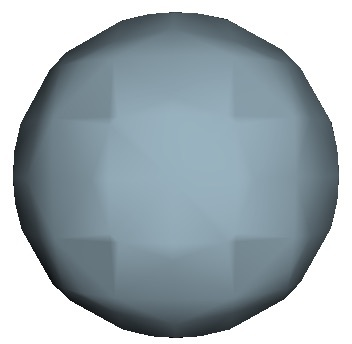
\includegraphics[width=7cm]{sphere_obj.jpg}
 %\end{center}
 \begin{figure}
\centering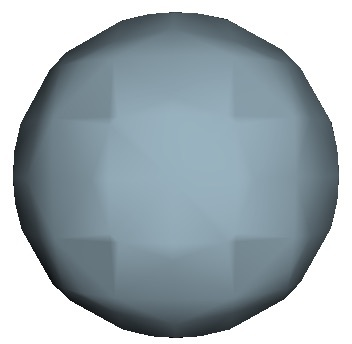
\includegraphics[width=7cm]{sphere_obj.jpg}
\caption{Original Sphere mesh}
\end{figure}
Figure 1 is that reads the mesh file, and displayed in OpenGL. This sphere is unit sphere. And This sphere have 174 vertices. Deform one point of this mesh.\\
 \begin{figure}
\centering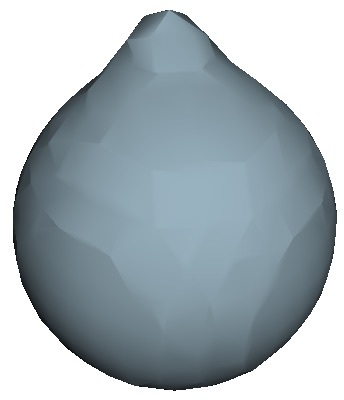
\includegraphics[width=7cm]{deformed_sphere_hrbf.jpg}
\caption{Deformed sphere(HRBF)}
\end{figure}
 \begin{figure}
\centering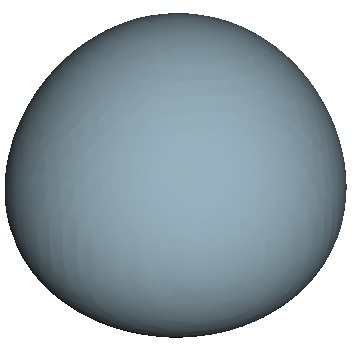
\includegraphics[width=7cm]{deformed_sphere_hrbfclosed.jpg}
\caption{Deformed sphere(Closed HRBF)}
\end{figure}
 \begin{figure}
\centering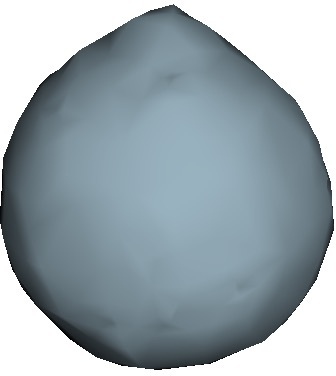
\includegraphics[width=7cm]{deformed_sphere_poisson.jpg}
\caption{Deformed sphere(Poisson surface reconstruction)}
\end{figure}
Figure 2 is that HRBF reconstruct deformed point cloud. Figure 3 is that Closed  HRBF surface reconstruction. Figure 4 is that Poisson surface reconstruction. HRBF is representing the smooth deformation. But HRBF slowest in three surface reconstructions. When the number of points increases, notebook PC takes too much time. Closed HRBF is faster than HRBF. But Closed HRBF is not precisely reconstructed. Poisson surface reconstruction is the fastest. Poisson surface reconstruction has been accurately reconstructed. However, detail is not smooth. 
\section{Conclusion}
% (4) Summarize what was done. Explain the parts that need further work and how you plan to extend this work in the future.
In this paper, we proposed program that have deformation algorithm that works by applying a field, corresponding to the deformation to the vertices of a triangle mesh, and three algorithm to reconstruct it. Our algorithm is not fast. It is possible to implement a more efficient way. Implementing part of the algorithm on the graphics card(GPU), using a modified meshing algorithm that tracks the surface, exploiting the locality of the deformation and compactly supported splines. 
\\ \ The first way to improve the efficiency of our approach is to implement the algorithm for fitting and evaluating the RBF as well as the meshing algorithm (the Marching Cubes) on the graphics card. One of the bottleneck of the current algorithm is the evaluation of the fitted function on the corners of every cell in the regular grid used by the Marching Cubes algorithm. It is possible to improve this approach by considering only the grid cells near the surface (this information is provided by the deformed point-cloud). 
\\ \ When compactly supported splines (the spline is non-zero on a compact set) are used in the HRBF approach(Closed HRBF), it does not seem necessary to recompute the function value at cells corners away from the deformed region. This should allow to further decrease the computational time when multiple deformations are applied on a given object.

\section*{Acknowledgement}
\section{Reference}
[1] Alexis Angelidis, Marie-Paule Cani, Geoff Wyvill, and Scott King. 2006. Swirling-sweepers: constant-volume modeling. Graph. Models 68, 4 (July 2006), 324-332.

[2] Robert Bridson. Computational aspects of dynamic surface. PhD. dissertation. Stanford. 2003.

[3] Mario Botsch, Leif Kobbelt, Mark Pauly, Pierre Alliez, and Bruno Levy. Polygon Mesh Processing.\\

[4] Macedo, Ives, Joao Paulo Gois, and Luiz Velho. �hHermite radial basis functions implicits.�h Computer Graphics Forum. Vol. 30. No. 1. Blackwell Publishing Ltd, 2011.\\

[5] Turk, Greg, and James F. O�fbrien. �hModelling with implicit surfaces that interpolate.�h ACM Transactions on Graphics (TOG) 21.4 (2002): 855-873.\\

[6] Lorensen, William E., and Harvey E. Cline. �hMarching cubes: A high resolution 3D surface construction algorithm.�h ACM siggraph computer graphics. Vol. 21. No. 4. ACM, 1987.\\

[7]  The Computational Geometry Algorithms Library http://www.cgal.org/ \\

[8]  Shengjun Liu, Charlie C. L. Wang, Senior Member, IEEE, Guido Brunnett, and Jun Wang "A Closed-Form Formulation of HRBF-Based Surface Reconstruction"

\bibliography{s1200045}


\end{document}
